\section{Supplementary Appendix}
\label{appx:internet-appendix}

% \subsection{Additional Estimator Definitions.}
% \label{appx:additional-estr-defs}
% Let $M \equiv I_n - P$ denote the residual projection matrix, with entry
% $M_{ij} = \mathbf{1}[i=j] - P_{ij}$, and let \(\tilde D\) and \(\tilde Y\) denote the stacked sample matrices of \(\tilde D_i\) and \(\tilde Y_i\), respectively.\footnote{This section is saved for posterity.}


% \begin{definitionp}{LIML}[LIML Estimator]\label{def:liml}
% Let $\hat\kappa$ denote the smaller root of
% \begin{align}
% \det\begin{pmatrix}
% \tilde Y'P\tilde Y - \kappa\, \tilde Y'M\tilde Y & \tilde D'P\tilde Y - \kappa\, \tilde D'M\tilde Y \\
% \tilde D'P\tilde Y - \kappa\, \tilde D'M\tilde Y & \tilde D'P\tilde D - \kappa\, \tilde D'M\tilde D
% \end{pmatrix} = 0.
% \label{eq:liml-eigenvalue}
% \end{align}
% The LIML estimator is defined as:
% \begin{align}
% \hat B_{\mathrm{LIML}} \equiv \frac{\tilde D'P\tilde Y - \hat\kappa\, \tilde D'M\tilde Y}{\tilde D'P\tilde D - \hat\kappa\, \tilde D'M\tilde D}.
% \label{eq:liml-def}
% \end{align}
% \end{definitionp}
% \begin{remark}
%     Setting $\hat\kappa = 0$ in \(\hat B_{LIML}\) recovers the TSLS estimator, $\hat B_{\mathrm{TSLS}}$.
% \end{remark}
% \noindent 
% The LIML estimator does not have a finite moment. The Fuller $k$ estimator ameliorates this by a correction term.
% \begin{definitionp}{FULK}[Fuller $k$ Estimator]\label{def:fuller}
% Let $\hat\kappa$ be defined as for the LIML estimator, and define
% $\hat\kappa_F(k) \equiv \hat\kappa - k/(n - d_Z)$.
% Then:
% \begin{align}
% \hat B_{\mathrm{FUL}(k)} \equiv \frac{\tilde D'P\tilde Y - \hat\kappa_F(k)\, \tilde D'M\tilde Y}{\tilde D'P\tilde D - \hat\kappa_F(k)\, \tilde D'M\tilde D}.
% \label{eq:fuller-def}
% \end{align}
% \end{definitionp}
% \begin{remark}
%     Standard choices for the tuning parameter \(k\) are $k=1$ and \(k=4\). The former gives an approximately median-unbiased estimator and finite moments of all orders. The latter produces an approximately MSE-minimizing estimator.
% \end{remark}

% \noindent
% Both the LIML and Fuller k estimators admit ``JIVE'' versions with  corrections that make the estimators consistent in the presence of heteroskedasticity (\citealp{hausmanInstrumentalVariableEstimation2012}, HLIM, HFUL). However, these obtain the same limiting distributions as LIML and Fuller k, hence we abstract from them in the present. 

% \begin{remark}
% TSLS, JIVE, LIML and Fuller k can all be written on the form:
% \begin{align*}
% \hat B = \frac{N - \xi\, \tilde N}{T - \xi\, \tilde{T}},
% \end{align*}
% where $(N, T)$ are cross-products from a projection, either with or without leaving out the diagonal elements, 

% and
% $(\tilde N, \tilde{T})$ are residualized cross-products weighted by $M_{ij}$ or $(1-P_{ii})$.
% The scalar $\xi$ is a data-dependent eigenvalue correction:
% \begin{center}
% \begin{tabular}{lll}
% \toprule
% Estimator & Correction $\xi$ & Base projection \\
% \midrule
% TSLS & $0$ & full ($P_{ij}$) \\
% LIML & $\hat\kappa$ & full \\
% Fuller($k$) & $\hat\kappa_F(k) = \hat\kappa - k/(n-d_Z)$ & full \\
% JIVE & $0$ & off-diagonal ($P_{ij}$, $i\neq j$)\\
% HLIM & $\hat\alpha_H$ & off-diagonal \\
% HFUL & $\hat\alpha_{HF} = \hat\alpha_H - c_n$ & off-diagonal \\
% \bottomrule
% \end{tabular}
% \end{center}

% \end{remark}

% \paragraph*{Bias of LIML, Fuller-k and TSLS-JIVE.}
% It is interesting to consider whether the combined TSLS-JIVE estimator obtains similar rates of relative bias as LIML and Fuller-k under the assumption of constant effects. In \Cref{fig:bias-jive-tsls-combined-all} we plot the bias of all four estimators. It is clear that the bias of the combined TSLS-JIVE estimator is closer to the LIML and Fuller-k estimators than to TSLS or JIVE. However, as the number of instruments increase, the bias of the combined estimator becomes more biased than LIML and Fuller-k as it drifts towards the bias of the JIVE estimator.


% \begin{figure}[!htb]
%     \centering
%     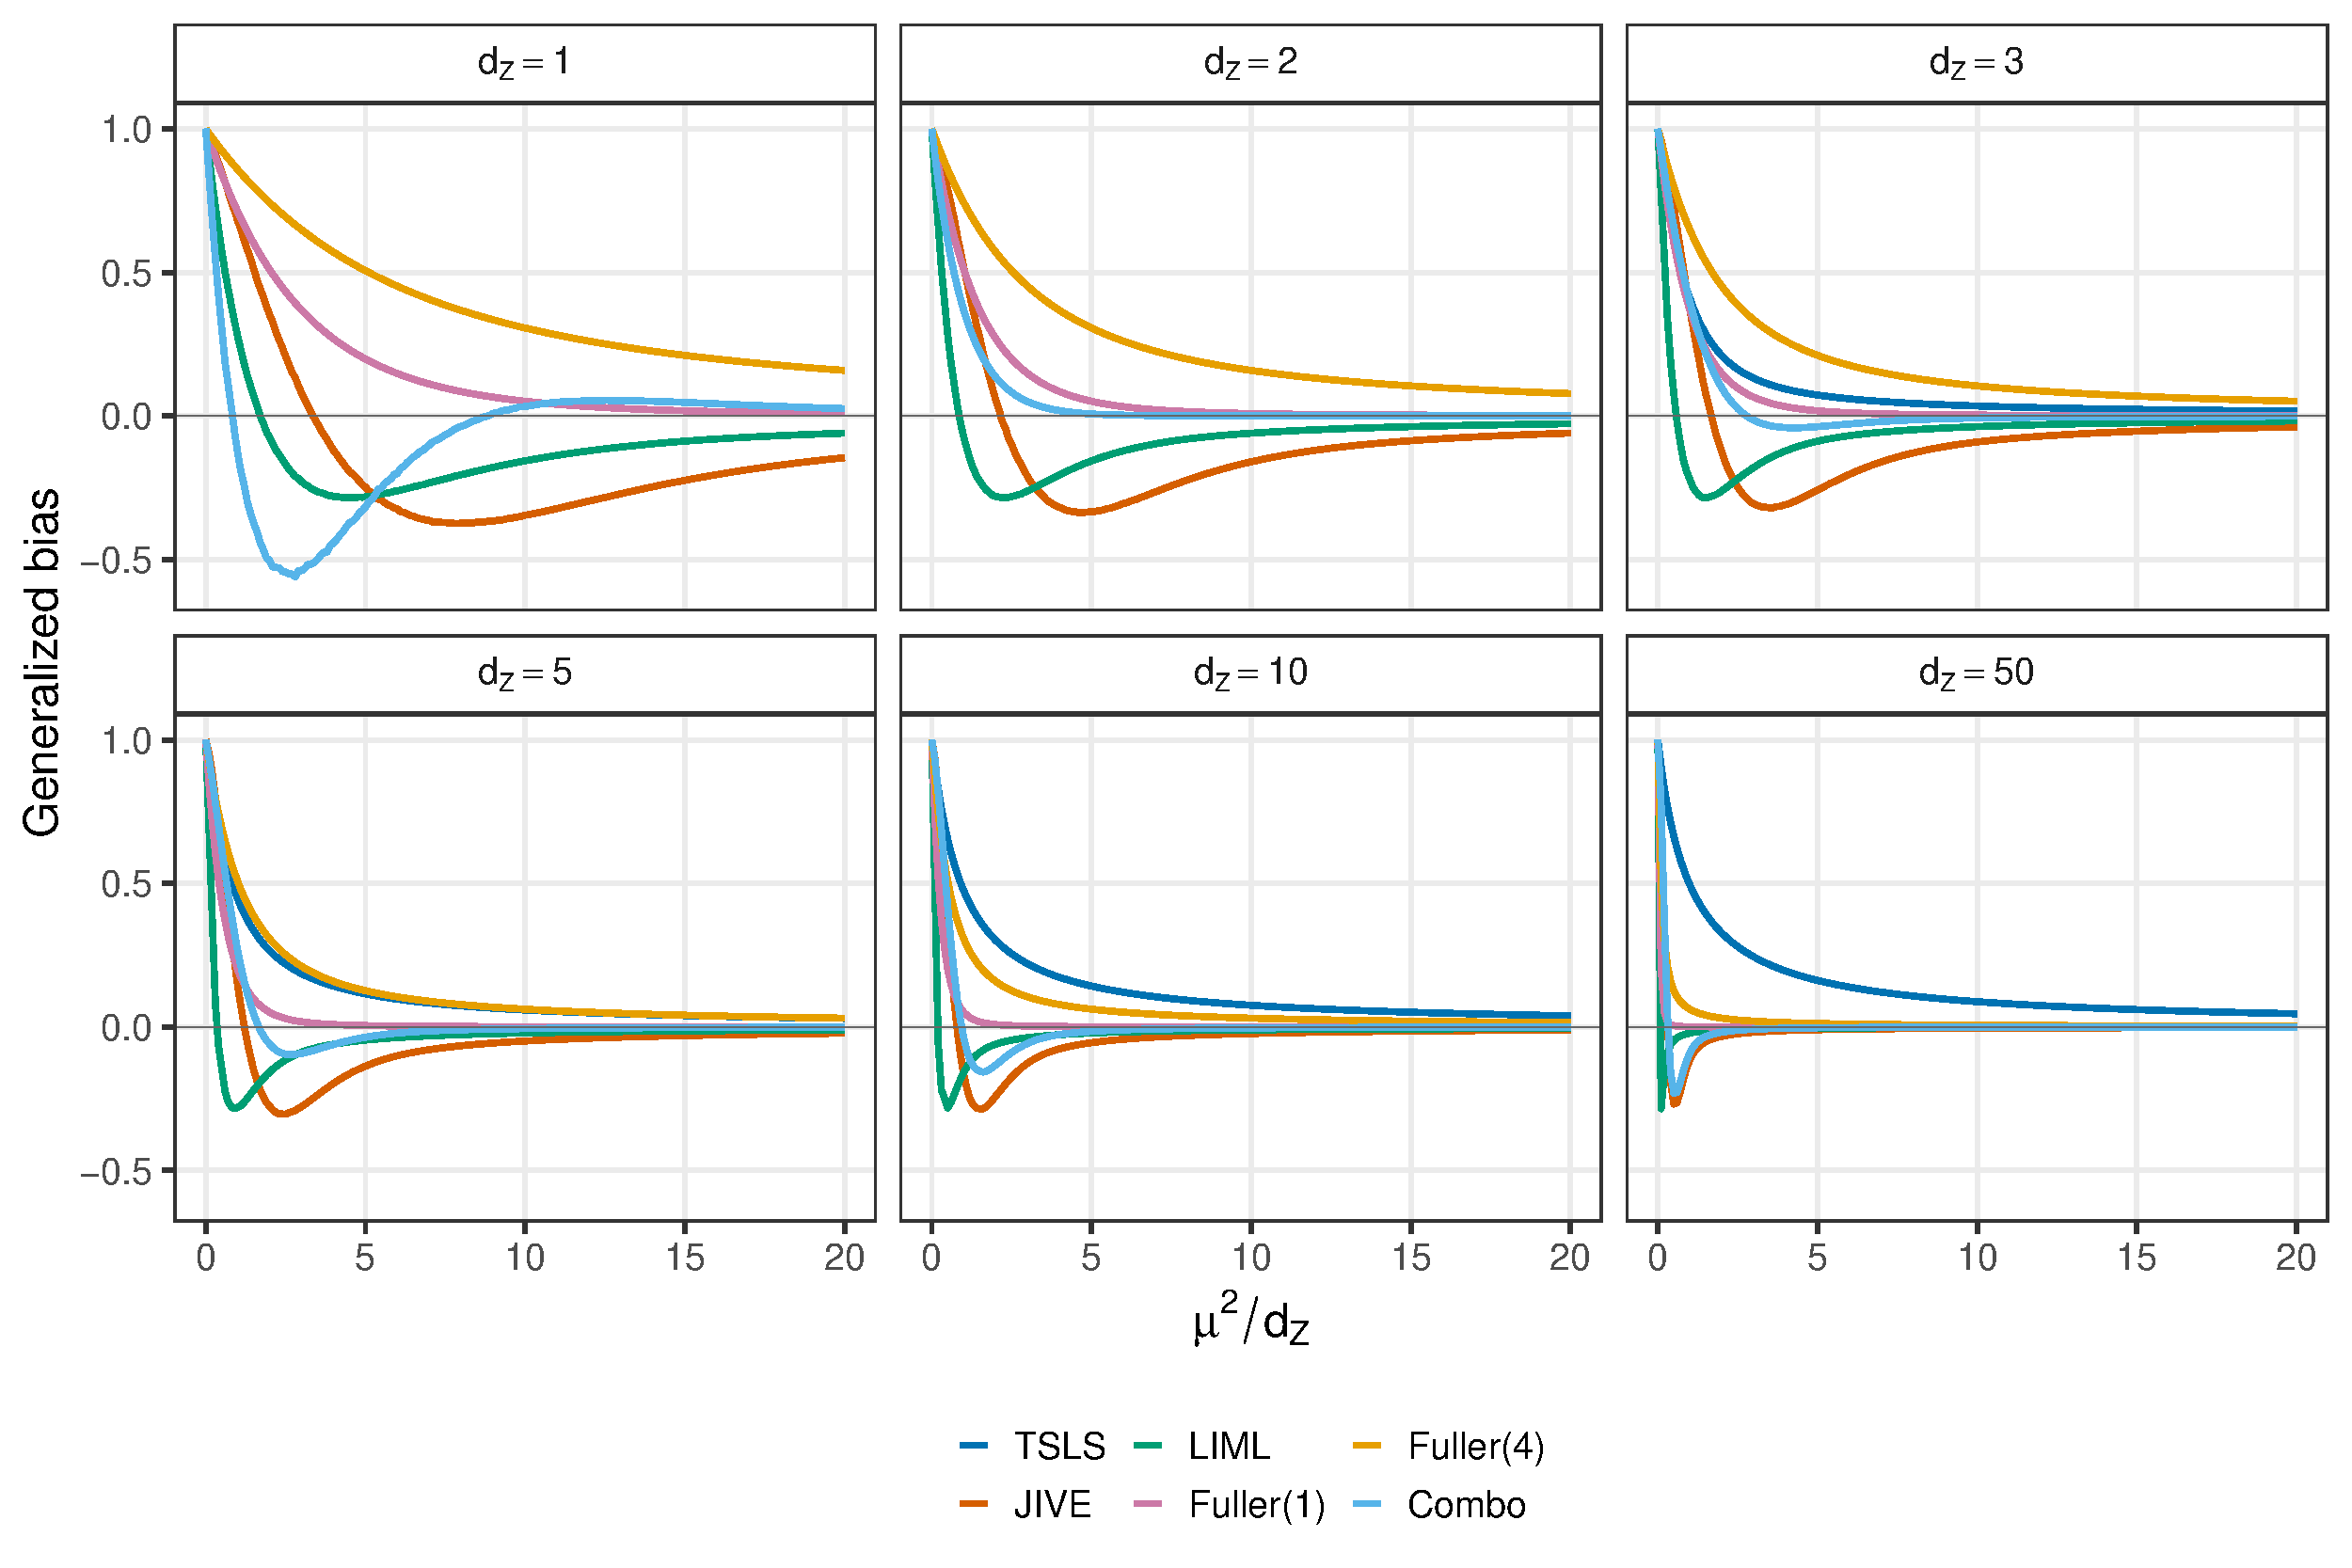
\includegraphics[width=\textwidth]{figs/limit_bias_all_estimators_by_dz.pdf}
%     \caption{\textbf{Generalized Bias of the Combined TSLS-JIVE Estimator and Other Alternative Estimators.} This figure shows 
%     the generalized bias of the combined TSLS-JIVE estimator for different numbers of instruments, \(d_Z\) and different values of the concentration parameter. Bias is shown as a function of \(\mu^2/d_Z\) which can be thought of as the average concentration of each instrument. The bias of the TSLS, JIVE, LIML and Fuller-k estimators are shown for comparison. Bias is shown relative to \(\omega\). 
%       }
%     \label{fig:bias-jive-tsls-combined-all}
% \end{figure}
